%%%%%%%%%%%%%%%%%%%%%%%%%%%%%%%%%%%%%%%%%
% Arsclassica Article
% LaTeX Template
% Version 1.0 (21/4/14)
%
% This template has been downloaded from:
% http://www.LaTeXTemplates.com
%
% Original author:
% Lorenzo Pantieri (http://www.lorenzopantieri.net) with extensive modifications by:
% Vel (vel@latextemplates.com)
%
% License:
% CC BY-NC-SA 3.0 (http://creativecommons.org/licenses/by-nc-sa/3.0/)
%
%%%%%%%%%%%%%%%%%%%%%%%%%%%%%%%%%%%%%%%%%

%----------------------------------------------------------------------------------------
%	PACKAGES AND OTHER DOCUMENT CONFIGURATIONS
%----------------------------------------------------------------------------------------
\documentclass[
10pt, % Main document font size
a4paper, % Paper type, use 'letterpaper' for US Letter paper
oneside, % One page layout (no page indentation)
%twoside, % Two page layout (page indentation for binding and different headers)
headinclude,footinclude, % Extra spacing for the header and footer
BCOR5mm, % Binding correction
]{scrartcl}

%%%%%%%%%%%%%%%%%%%%%%%%%%%%%%%%%%%%%%%%%
% Arsclassica Article
% Structure Specification File
%
% This file has been downloaded from:
% http://www.LaTeXTemplates.com
%
% Original author:
% Lorenzo Pantieri (http://www.lorenzopantieri.net) with extensive modifications by:
% Vel (vel@latextemplates.com)
%
% License:
% CC BY-NC-SA 3.0 (http://creativecommons.org/licenses/by-nc-sa/3.0/)
%
%%%%%%%%%%%%%%%%%%%%%%%%%%%%%%%%%%%%%%%%%

%----------------------------------------------------------------------------------------
%	REQUIRED PACKAGES
%----------------------------------------------------------------------------------------

\usepackage[
nochapters, % Turn off chapters since this is an article        
beramono, % Use the Bera Mono font for monospaced text (\texttt)
eulermath,% Use the Euler font for mathematics
pdfspacing, % Makes use of pdftex’ letter spacing capabilities via the microtype package
dottedtoc % Dotted lines leading to the page numbers in the table of contents
]{classicthesis} % The layout is based on the Classic Thesis style

\usepackage{arsclassica} % Modifies the Classic Thesis package

\usepackage[T1]{fontenc} % Use 8-bit encoding that has 256 glyphs

\usepackage[utf8]{inputenc} % Required for including letters with accents

\usepackage{graphicx} % Required for including images
\graphicspath{{Figures/}} % Set the default folder for images

\usepackage{enumitem} % Required for manipulating the whitespace between and within lists

\usepackage{lipsum} % Used for inserting dummy 'Lorem ipsum' text into the template

\usepackage{subfig} % Required for creating figures with multiple parts (subfigures)

\usepackage{amsmath,amssymb,amsthm} % For including math equations, theorems, symbols, etc

\usepackage{varioref} % More descriptive referencing


%----------------------------------------------------------------------------------------
%	THEOREM STYLES
%---------------------------------------------------------------------------------------

\theoremstyle{definition} % Define theorem styles here based on the definition style (used for definitions and examples)
\newtheorem{definition}{Definition}

\theoremstyle{plain} % Define theorem styles here based on the plain style (used for theorems, lemmas, propositions)
\newtheorem{theorem}{Theorem}

\theoremstyle{remark} % Define theorem styles here based on the remark style (used for remarks and notes)

%----------------------------------------------------------------------------------------
%	HYPERLINKS
%---------------------------------------------------------------------------------------

\hypersetup{
%draft, % Uncomment to remove all links (useful for printing in black and white)
colorlinks=true, breaklinks=true, bookmarks=true,bookmarksnumbered,
urlcolor=webbrown, linkcolor=RoyalBlue, citecolor=webgreen, % Link colors
pdftitle={}, % PDF title
pdfauthor={\textcopyright}, % PDF Author
pdfsubject={}, % PDF Subject
pdfkeywords={}, % PDF Keywords
pdfcreator={pdfLaTeX}, % PDF Creator
pdfproducer={LaTeX with hyperref and ClassicThesis} % PDF producer
} % Include the structure.tex file which specified the document structure and layout
\hyphenation{Fortran hy-phen-ation} % Specify custom hyphenation points in words with dashes where you would like hyphenation to occur, or alternatively, don't put any dashes in a word to stop hyphenation altogether

%----------------------------------------------------------------------------------------
%	TITLE AND AUTHOR(S)
%----------------------------------------------------------------------------------------

\title{\normalfont\spacedallcaps{Sub-Jupiter Radius Occurrence Rate Anomaly}} % The article title

\author{\spacedlowsmallcaps{Joe Renaud}} % The article author(s) - author affiliations need to be specified in the AUTHOR AFFILIATIONS block

\date{} % An optional date to appear under the author(s)

%----------------------------------------------------------------------------------------

\begin{document}

%----------------------------------------------------------------------------------------
%	HEADERS
%----------------------------------------------------------------------------------------

\renewcommand{\sectionmark}[1]{\markright{\spacedlowsmallcaps{#1}}} % The header for all pages (oneside) or for even pages (twoside)
%\renewcommand{\subsectionmark}[1]{\markright{\thesubsection~#1}} % Uncomment when using the twoside option - this modifies the header on odd pages
\lehead{\mbox{\llap{\small\thepage\kern1em\color{halfgray} \vline}\color{halfgray}\hspace{0.5em}\rightmark\hfil}} % The header style

\pagestyle{scrheadings} % Enable the headers specified in this block

%----------------------------------------------------------------------------------------
%	TABLE OF CONTENTS & LISTS OF FIGURES AND TABLES
%----------------------------------------------------------------------------------------

\maketitle % Print the title/author/date block

\setcounter{tocdepth}{2} % Set the depth of the table of contents to show sections and subsections only

\tableofcontents % Print the table of contents

\listoffigures % Print the list of figures

\listoftables % Print the list of tables

%----------------------------------------------------------------------------------------
%	ABSTRACT
%----------------------------------------------------------------------------------------

\section*{Abstract} % This section will not appear in the table of contents due to the star (\section*)

%----------------------------------------------------------------------------------------
%	AUTHOR AFFILIATIONS
%----------------------------------------------------------------------------------------

%\let\thefootnote\relax\footnotetext{* \textit{Department of Biology, University of Examples, London, United Kingdom}}

%\let\thefootnote\relax\footnotetext{\textsuperscript{1} \textit{Department of Chemistry, University of Examples, London, United Kingdom}}

%----------------------------------------------------------------------------------------

\newpage % Start the article content on the second page, remove this if you have a longer abstract that goes onto the second page

%----------------------------------------------------------------------------------------
%	INTRODUCTION
%----------------------------------------------------------------------------------------

\section{Introduction}

Since the first confirmation of an extra-solar planet in 1992\cite{Wolszczan:1992}, the field of exoplanet research has exploded with nearly 1800 planets currently confirmed (as of May 6th, 2014\cite{ExoData:nasa}). Since the early 90's the detection techniques employed to discover these exoplanets relied heavily upon tracking the Doppler shift in a host star's spectrum. Such a shift could arise from a large, short period, exoplanet. The radial velocity technique formed the majority of exoplanet confirmations well into the late 2000's\cite{RV1}. During this time the transit technique started to gain prevalence. 
\subsection{Transit Technique and NASA's Kepler Mission}
Exoplanet transiting refers to the event when a exoplanet passes into the line of sight of the observer to the host star. A host star's light can be monitored over a certain time span; when compared to the light output of similar stars in the same frame - a exoplanet detection can be easily picked out (see figure~\vref{fig:transit}). These light curves allow researchers to determine certain characteristics of the transiting planet. Specifically from one transit one can find the ratio of the radius of the planet compared to the host star. Multiple transits will provide orbital information\cite{TR1}.
\begin{figure}[tb]
\centering 
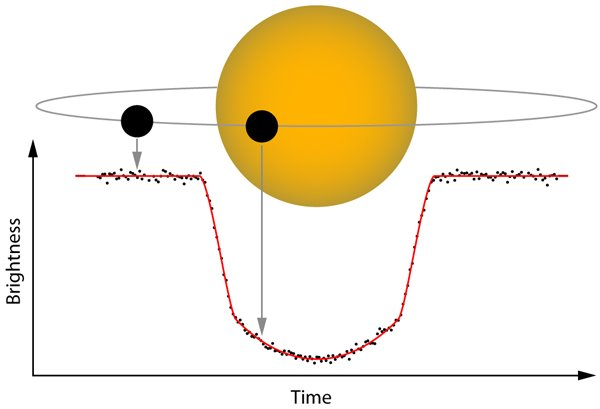
\includegraphics[width=0.5\columnwidth]{transit} 
\caption[Transiting Exoplanet]{Cartoon of a transiting exoplanet, image taken from NASA exoplanet database}
\label{fig:transit} 
\end{figure}
The early days of transit discoveries found only large radius planets as these required the least sensitive equipment, and from the fact that the signal to noise ratio of an exoplanet discovery is described by equations 1 and 2. 
\begin{equation}
\frac{S}{N} \approx \sqrt{N_{t}}\frac{\delta}{\sigma}
\label{eq:t1}
\end{equation}
\begin{equation}
\delta = \left(\frac{R_{p}}{R_{*}}\right)^{2}
\label{eq:t2}
\end{equation}
The radius of the planet $R_{p}$ and the radius of the star $R_{*}$ greatly impacts the S/N, as does the photometric precision $\sigma$\cite{DST}. Thus, these early discoveries had limited (and small) photometric precision. Therefore, the only planets that had a decent signal to noise ratio were those with large radii. This can be seen in the histogram of radii for all exoplanets discovered by the transit technique up to 2008 (Figure~\vref{fig:transit2}). Jupiter size planets and larger were common discoveries for the transit technique. It was not until NASA's Kepler mission was launched in 2009\cite{kep2} that photometric precision was increased to the point that sub-Jupiter planets could be detected\cite{kep1}. Once Kepler's data began getting published it became clear that not only could Kepler detect planets down to the sub-Earth size, but it was also able to find planets much more quickly - increasing the exoplanet database size dramatically (Figure~\vref{fig:transit2}). There are over 1700 exoplanets discovered through the transit, and other techniques (last checked on May 10th 2014\cite{ExoData:nasa}). All of these planets provide a good sampling of the potential exoplanets within our galaxy. There has been a number of studies that examine properties of the currently discovered exoplanets (e.g: \cite{occ1,Marcey1,occ2}). This project examines an anomaly in the distribution of exoplanet radii in transiting exoplanets.
\begin{figure}[tb]
\centering 
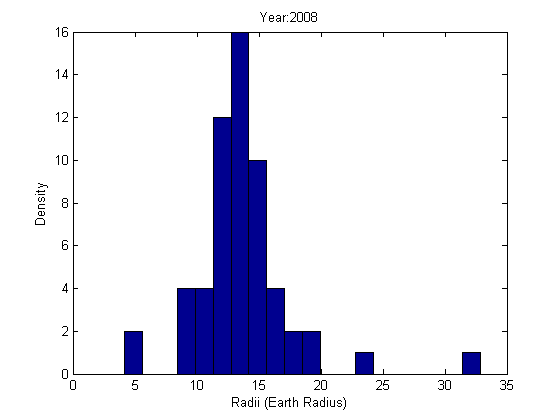
\includegraphics[width=0.8\columnwidth]{2008TransitRadius} 
\caption[>2008 Exoplanet transit discoveries]{Exoplanet discoveries made by the transiting technique from 1990 to 2008. The radii are measured in Earth Radii, with ~10 Earth Radius being roughly the size of Jupiter.}
\label{fig:transit2} 
\end{figure}
\begin{figure}[tb]
\centering 
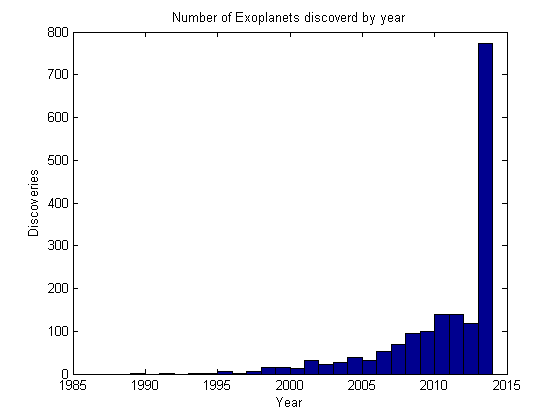
\includegraphics[width=0.8\columnwidth]{2014Transit} 
\caption[Current Transit Technique Discoveries]{Transit technique discoveries up to April 25th 2014. It is clear that since Kepler's launch in 2009, the exoplanet database has grown substantially.}
\label{fig:transit2} 
\end{figure}
\subsection{Radii of Discovered Planets}
We are specifically curious what the distribution of exoplanet radius has been changing since the introduction of the Kepler mission. Since radius is a primary variable of only the transit technique: most of the analysis will be based upon planets discovered by transiting. However, some planets originally discovered by radial velocity, or other techniques, have been reexamined by telescopes using the transit technique. This allows some analysis of radii of radial velocity exoplanets. 


 
%----------------------------------------------------------------------------------------
%	METHODS
%----------------------------------------------------------------------------------------
\section{Data}
The data for this study is obtained from \href{"http://exoplanetarchive.ipac.caltech.edu/cgi-bin/ExoTables/nph-exotbls?dataset=planets"}{NASA Confirmed Exoplanet Database} and 
\href{"http://exoplanetarchive.ipac.caltech.edu/cgi-bin/ExoTables/nph-exotbls?dataset=cumulative"}{NASA Exoplanet Candidate Database}. This data is updated continuously by the scientific community and managed by NASA, making it a very reliable source. The specific type of data that can be pulled from this source includes publication date, Planetary properties (mass, radius, period, etc), Stellar properties (mass, radius, galactic location, etc), and detection information. A number of planets detected by the transit method up to the current date can be found on figure~\vref{fig:transit2}. To ensure reliability of data: any exoplanet that was examined was first cross referenced on a different, but still well cited, exoplanet database - \href{"http://exoplanets.eu/"}{Exoplanets.eu}. Specifically, planet radii were confirmed to be the same across both databases. Any planet that had a significant variation across the sources was neglected from the study. 

Issues with this data is that the date listed does not necessarily correspond to the date when technology was sufficient enough to detect said planet, but rather when enough research and/or follow-ups were preformed to make a publication regarding its discovery. This means that the capability of discovering does not scale with publication year. This means that predictions as to when technology will be sufficient enough to detect a planet of a certain radius ( $P(R)\propto{}R^{n}$ ) can not be easily extrapolated. 
\section{Methods}

Reference to Figure~\vref{fig:gallery}. % The \vref command specifies the location of the reference

\begin{figure}[tb]
\centering 
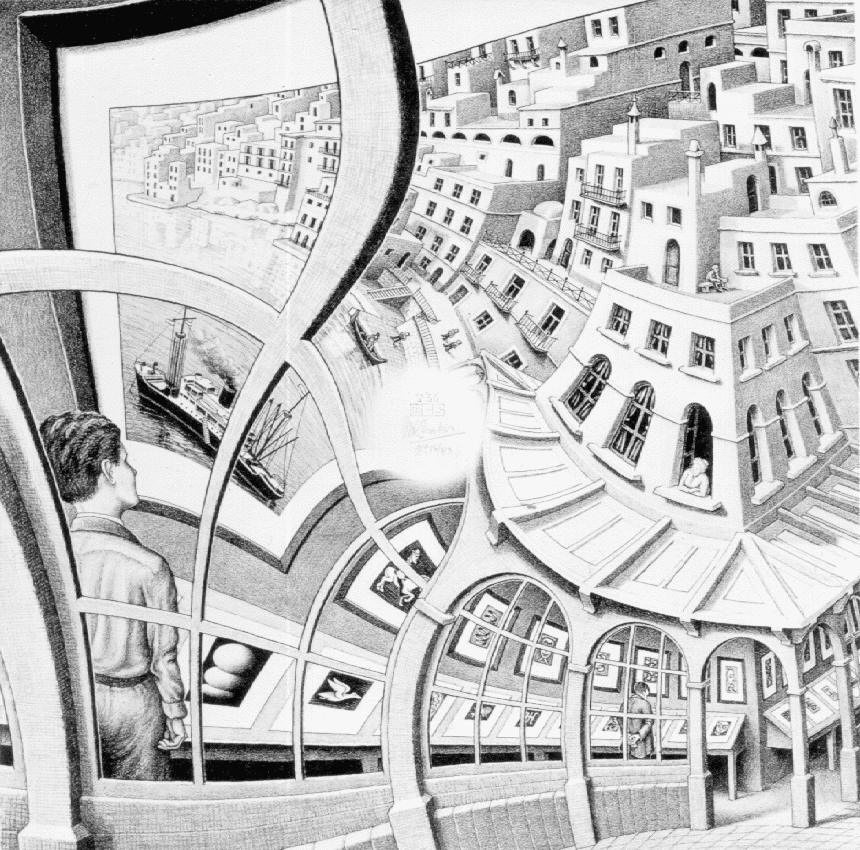
\includegraphics[width=0.5\columnwidth]{GalleriaStampe} 
\caption[An example of a floating figure]{An example of a floating figure (a reproduction from the \emph{Gallery of prints}, M.~Escher,\index{Escher, M.~C.} from \url{http://www.mcescher.com/}).} % The text in the square bracket is the caption for the list of figures while the text in the curly brackets is the figure caption
\label{fig:gallery} 
\end{figure}

\lipsum[5] % Dummy text

\begin{enumerate}[noitemsep] % [noitemsep] removes whitespace between the items for a compact look
\item First item in a list
\item Second item in a list
\item Third item in a list
\end{enumerate}

%------------------------------------------------

\subsection{Paragraphs}

\lipsum[6] % Dummy text

\paragraph{Paragraph Description} \lipsum[7] % Dummy text

\paragraph{Different Paragraph Description} \lipsum[8] % Dummy text

%------------------------------------------------

\subsection{Math}

\lipsum[4] % Dummy text

\begin{equation}
\cos^3 \theta =\frac{1}{4}\cos\theta+\frac{3}{4}\cos 3\theta
\label{eq:refname2}
\end{equation}

\lipsum[5] % Dummy text

\begin{definition}[Gauss] 
To a mathematician it is obvious that
$\int_{-\infty}^{+\infty}
e^{-x^2}\,dx=\sqrt{\pi}$. 
\end{definition} 

\begin{theorem}[Pythagoras]
The square of the hypotenuse (the side opposite the right angle) is equal to the sum of the squares of the other two sides.
\end{theorem}

\begin{proof} 
We have that $\log(1)^2 = 2\log(1)$.
But we also have that $\log(-1)^2=\log(1)=0$.
Then $2\log(-1)=0$, from which the proof.
\end{proof}

%----------------------------------------------------------------------------------------
%	RESULTS AND DISCUSSION
%----------------------------------------------------------------------------------------

\section{Results and Discussion}

\lipsum[10] % Dummy text

%------------------------------------------------

\subsection{Subsection}

\lipsum[11] % Dummy text

\subsubsection{Subsubsection}

\lipsum[12] % Dummy text

\begin{description}
\item[Word] Definition
\item[Concept] Explanation
\item[Idea] Text
\end{description}

\lipsum[12] % Dummy text

\begin{itemize}[noitemsep] % [noitemsep] removes whitespace between the items for a compact look
\item First item in a list
\item Second item in a list
\item Third item in a list
\end{itemize}

\subsubsection{Table}

\lipsum[13] % Dummy text

\begin{table}[hbt]
\caption{Table of Grades}
\centering
\begin{tabular}{llr}
\toprule
\multicolumn{2}{c}{Name} \\
\cmidrule(r){1-2}
First name & Last Name & Grade \\
\midrule
John & Doe & $7.5$ \\
Richard & Miles & $2$ \\
\bottomrule
\end{tabular}
\label{tab:label}
\end{table}

Reference to Table~\vref{tab:label}. % The \vref command specifies the location of the reference

%------------------------------------------------

\subsection{Figure Composed of Subfigures}

Reference the figure composed of multiple subfigures as Figure~\vref{fig:esempio}. Reference one of the subfigures as Figure~\vref{fig:ipsum}. % The \vref command specifies the location of the reference

\lipsum[15-18] % Dummy text

\begin{figure}[tb]
\centering
\subfloat[A city market.]{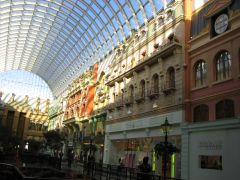
\includegraphics[width=.45\columnwidth]{Lorem}} \quad
\subfloat[Forest landscape.]{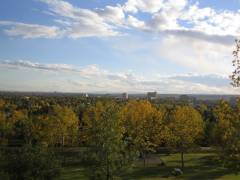
\includegraphics[width=.45\columnwidth]{Ipsum}\label{fig:ipsum}} \\
\subfloat[Mountain landscape.]{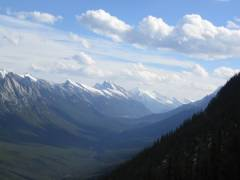
\includegraphics[width=.45\columnwidth]{Dolor}} \quad
\subfloat[A tile decoration.]{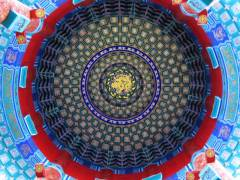
\includegraphics[width=.45\columnwidth]{Sit}}
\caption[A number of pictures.]{A number of pictures with no common theme.} % The text in the square bracket is the caption for the list of figures while the text in the curly brackets is the figure caption
\label{fig:esempio}
\end{figure}

%----------------------------------------------------------------------------------------
%	BIBLIOGRAPHY
%----------------------------------------------------------------------------------------

\renewcommand{\refname}{\spacedlowsmallcaps{References}} % For modifying the bibliography heading

\bibliographystyle{plain}
%\bibliographystyle{apa}

\bibliography{DocumentR} % The file containing the bibliography

%----------------------------------------------------------------------------------------

\end{document}